\chapter{Tracking cancer evolution \textit{in silico} via evolutionary
indices}\label{chapter:trajectories}


\section{Introduction}
A trajectory is a path described by any object (or indeed point) in some space
according to some parameter, usually time.  Intuitively then, an evolutionary
trajectory refers to the changes that a lineage or population undergoes over
time --- the series of genetic, morphological, and behavioral transformations
that occur as organisms evolve and diversify. I am interested in the
evolutionary trajectory of cancers but reliably obtaining time-series data is,
at the time of writing, not feasible at a larger scale. This stems from multiple
issues. Firstly, at time of diagnosis, solid tumours have likely already been
growing for long enough to reach a size visible in standard medical imaging
\cite{patrone_how_2011}. This means that even initial data obtained in the
clinic represents a relatively late stage in the cancer's evolutionary history
most of the time. Secondly, solid tumours are just that --- clumps of cells
organised in some way in space --- meaning that taking a sample from one point
in the tumour is not necessarily representative of the rest of the cell
population. Finally, a biopsy is an invasive procedure which can cause
considerable discomfort to patients, depending on where the tumour is situated.
Therefore, having a reasonable estimate of a tumours evolutionary trajectory
based on the data that is available at time of sequencing would allow for a more
informed treatment strategy. This begs the question --- how can we distinguish
between different ways tumours evolve? Is it necessary to wade through sequences
of genetic data to do so or is it possible to abstract the key properties of a
tumour's evolutionary trajectory into a few numerical summaries? \par In this
chapter, I will examine the utility of two different sets of evolutionary
indices for tracking the evolution of tumours on the example of agent-based
simulations.


\section{Preliminaries}

\subsection{Modes of evolution}
Over the years, there have been a number of different definitions of what a mode
of evolution is. Initially, it was introduced as the term which covers the way
or manner in which a species evolves \cite{eiseley_tempo_1945}. Depending on the
piece of literature, it could also refer to the model used in the study of a
population's evolutionary trajectory \cite{yotoko_does_2011}, or the mechanism
which drives the evolution such as genetic drift \cite{glassman_cancer_1996,
wolf_genome_2013}. This ambiguity of terminology is present in cancer research
as well. In this thesis, I will use the term mode of evolution as originally
defined by \cite{eiseley_tempo_1945}, and used by \cite{davis_tumor_2017,
noble_spatial_2022}. That is, the way in which a tumour evolves (figure
\ref{fig:modes}).

\begin{figure}[h!]
    \centering
    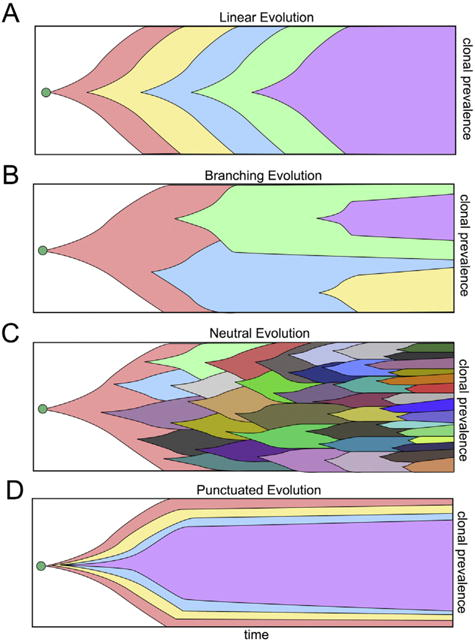
\includegraphics[width=0.85\textwidth]{Chapter_3/figures/modes.jpeg}
    \caption{Four different modes of tumour evolution. Picture adapted from
    \cite{davis_tumor_2017} under a CC BY 4.0 license.}
    \label{fig:modes}
\end{figure}

\subsection{Why even bother with indices?}
Before introducing the sets of indices used to analyse properties of trees, let
us consider a simpler question --- is it possible map the set of all possible
trees to the set of real numbers? For this purpose I had to decide how to
define the set of trees. The number of nodes in a tree is a natural number,
$n\in\mathbb{N}$, as is the number of possible tree topologies for a given $n$.
We denote with $T(n)$ the set of enumerated tree topologies
\cite{nakano_tree_2016}. Each node then has a corresponding size, giving us an
$n$-tuple of real numbers $(\alpha_1, \dots, \alpha_n)\in\mathbb{R}^n$, and
each edge (branch) has a corresponding length or $(l_i, \dots,
l_{(n-1)})\in\mathbb{R}^{(n-1)}$. This means we would need a family of maps

\begin{equation}
    f_n: A(n) \times \mathbb{R}^n \times \mathbb{R}^{n-1} \rightarrow R.
\end{equation}

It would be easy to construct a mapping which would allow us to ``enumerate"
each possible tree with a real number. The problem with this approach, however,
is that it would not be very informative. The real numbers are not ordered in
any way that would allow us to meaningfully compare trees. The lack of
interpretability would render any application of such a mapping useless. This is
where tree shape indices come in as a way to summarise key properties of a tree
in a way that is both interpretable and mathematically sound.

\subsection{A 3-dimensional index space --- trees with uniform branch lengths}

\subsubsection{Shannon diversity}
Shannon entropy is a fundamental concept in information theory, that quantifies
the uncertainty or randomness of a system \cite{shannon_mathematical_1948}. By
considering a system where diversity represents the variety of elements, such as
intra-tumour heterogeneity, we can define the Shannon diversity as the
exponential of the Shannon entropy,

\begin{equation}
    \leftindex[I]^1{D} = \exp\left[\leftindex[I]^1{H}\right] =
    \exp\left[-\sum_{i=1}^N p_i \log p_i\right],
\end{equation}

where $N$ is the total number of categories (or elements, species, etc.), and
$p_i$ the frequency of category $i$. The Shannon diversity was chosen because of
the nice property that it is maximised and equal to the number of categories
when all categories are equally represented, and minimised when only one
category is present. Previous work on a similar topic \cite{noble_spatial_2022}
was based on the Simpson index \cite{simpson_measurement_1949}. However, the
Shannon index was chosen for this work because it is more sensitive to changes
in the frequencies of subclones, better interpretability, and the fact that the
$J^1$ index is based on the Shannon entropy.

\subsubsection{Mean number of drivers per cell --- distance from the root}
Each speciation event in phylogenetics or driver mutation in cancer evolution is
associated with a change in the corresponding tree's topology. To capture the
average number of these events, I use the mean number of drivers per cell. This
is defined as the average of distances from all nodes to the root (with the root
distance from itself defined as $1$) weighted by the frequencies of the
subclones,

\begin{equation}
    n = \sum_{i=1}^N p_i \nu(i),
\end{equation}

where $\nu(i)$ is the root distance of node $i$.

\subsubsection{Balance index}
As discussed in chapter \ref{chapter:trees}, the balance index $J^1$ is a
weighted average of the evenness of the population distribution within a tree.
We use it as the third index in this space.

\subsection{A general set of indices --- any rooted tree}
Expanding upon the $3$-dimensional space defined above, a new comprehensive set
of interpretable robust indices based on Hill numbers was introduced recently
\cite{noble_new_2023}. The authors expanded and improved upon the existing
quantifiers of tree shape properties by deriving methods for trees with
arbitrary node size, node degree, and branch length distributions. The methods
for calculating all of the indices are included as part of an R package
\cite{kimverity_kimverityruiindices_2023}.\par Each generalised index has three
components, depending on which part of the tree it is applied --- the
longitudinal mean, node-wise mean, star mean.

\subsubsection{Richness --- $\leftindex[I]^0{D}$}
Richness in the context of phylogenetics is simply the number of extant species,
i.e. the number of tips in a phylogenetic tree. The generalised richness's
three components are:

\begin{enumerate}
    \item $\leftindex[I]^0{D}_L$ --- the average number of branches across the
        tree;
    \item $\leftindex[I]^0{D}_N$ --- the average effective outdegree, ignoring
        branch sizes;
    \item $\leftindex[I]^0{D}_S$ --- the
        effective number of non-root nodes.
\end{enumerate}

\subsubsection{Diversity --- $\leftindex[I]^q{D}$, $q>0$}
The generalised diversity index represents an extension of the Shannon diversity
index. Its three components are:

\begin{enumerate}
    \item $\leftindex[I]^q{D}_L$ --- the effective number of maximally distant
        nodes (leaves);
    \item $\leftindex[I]^q{D}_N$ --- the average effective outdegree, accounting
        for branch sizes, i.e. bushiness;
    \item $\leftindex[I]^q{D}_S$ --- the effective numbering of branches,
        accounting for branch sizes.
\end{enumerate}

\subsubsection{Evenness --- $\leftindex[I]^q{J}$, $q>0$}
Finally, the extension of the robust universal balance index $J^1$, this set of
indices generalises tree balance in the following way:

\begin{enumerate}
    \item $\leftindex[I]^q{J}_L$ --- evenness of branch sizes across the tree,
        or tree symmetry for leafy and ultrametric trees;
    \item $\leftindex[I]^q{J}_N$ --- tree balance, or evenness of the node size
        distribution;
    \item $\leftindex[I]^q{J}_S$ --- evenness of all branch sizes.
\end{enumerate}


\section{Tree resolution}

I rejected the idea of simply mapping trees to real numbers due to the lack of
interpretability. Tree shape indices are nominally better, as they summarise
properties of a tree, but they may have limitations in the form of a lack of
resolution for certain types of trees. \par
Starting simple, we examine leafy trees with all leaves of equal size in the
$3$-dimensional index space. The first thing to note is that the Shannon
diversity will simply equal the number of leaves in the tree. This already takes
away a degree of freedom. The next thing to consider is the value of $J^1$. If
we limit our search, for now, to perfectly balanced trees, we are left with
symmetric trees on a fixed number of leaves $N$. To make the final index equal
between two trees, they need to have equal average depths of their leaves. As we
are only looking at perfectly symmetric trees, that means that the average depth
will be exactly equal to the individual leaf depths. We can then show the
following
\begin{proposition}
    Let $T$ be a symmetric leafy tree on $N$ leaves with equal leaf sizes. If
    the canonical factorisation of $N$ is
    \begin{equation}
        N = \prod_{i=1}^k \alpha_i^{l_i},
    \end{equation}
    then there are
    \begin{equation}
            \frac{\left(\sum^k_{i=1}l_i\right)!}{\prod_{i=1}^k l_i!}
    \end{equation}
    distinct trees with the same values of $J^1$, $\leftindex[I]^1{D}$, and $n$,
    including $T$.
\end{proposition}
\begin{proof}
    First, the values of indices $J^1$ and $D$ for a symmetric leafy tree with
    $N$ equally-sized leaves are
    \begin{align*}
        J^1 &= 1, \\
        D &= N, \\
        n &= 1 + \sum_{i=1}^k l_i.
    \end{align*}
    The result is then a simple combinatorial problem of placing $n-1$ balls
    ($\alpha_i$'s) into $n-1$ bins, with each $\alpha_i$ repeated $l_i$ times.
    Therefore, the number of distinct trees is
    \begin{equation}
        \frac{\left(\sum^k_{i=1}l_i\right)!}{\prod_{i=1}^k l_i!}.
    \end{equation}
\end{proof}

This case may be interesting mathematically, but is not too relevant for
practical purposes as it is highly unlikely that sequencing data would yield a
perfectly symmetric leafy tree. As the space of trees is so large, there is
little point in performing a grid search, especially when arbitrary node sizes
are considered. In testing, there have been no cases of trees with the same
values of indices, but different topologies. This is a good sign, as it means
that the indices are able to distinguish between different trees. However, the
question remains whether there is a set of indices which can differentiate
between any two trees.

\section{Computational methods}

\subsection{Agent-based modelling framework - \textit{warlock/demon}}
There is no shortage of agent-based models of tumour evolution
\cite{colyer_seven-step_2023}, and the can range from purpose-built complex
frameworks to more stripped-down and abstract ones. Since each model should be
``as simple as possible but no simpler", the appropriate framework for our
purposes must satisfy certain requirements --- flexibility, efficiency, and
reproducibility. The first requirement is deceptively specific. As the main
inspiration behind this work stems from cancer evolution, I wanted the
simulations to have parameters for controlling aspects of the cell population's
physical properties which would in turn imply a different way in which it
evolves. This would, for example, include spatial arrangement of cells, mutation
rates, migration rates, and selective advantage. Furthermore, while the goal is
to simulate large populations of cells, I also need a large number of
simulations over which more general deterministic properties can be deduced.
Stochastic effects could make vastly different evolutionary modes look more
similar than expected in theory. Finally, reproducibility allows us to share
parameters of our models for verification by peers, and possible further
investigation.\par
The agent-based modelling framework I decided to use is \texttt{warlock}
\cite{bak_warlock_2023}, a \texttt{snakemake} wrapper written for \texttt{demon}
\cite{noble_demon_2020}. It satisfies the requirements above, with a few
associated comments. Firstly, it is a flexible agent-based model of tumour
evolution as it does have parameters which control for spatial arrangement,
mutation rates and selective advantage, as well as migration. While it is able
to simulate spatial structure, \texttt{demon} covers at most two spatial
dimensions. This is not an issue since we approximate the cell population to
undergo stochastic isotropic growth, that is the tumour has equal probability of
expanding in all directions in space. This implies approximate spherical
symmetry of simulated solid tumours, which allows us to effectively consider the
two-dimensional simulation as a cross-section of a tumour spheroid. In terms of
efficiency, \texttt{demon} was written mainly in C++, and conceptualised so that
instead of tracking individual cells, it simulates unique cell genotypes on a
two-dimensional grid comprised of demes, or well-mixed patches of cells. The
procedure for simulation cell events is based on the Gillespie algorithm
\cite{gillespie_exact_1977}, and follows the steps of selecting a deme, then
cell type, event type, and finally cell genotype. This approach sacrifices
micro-scale interactions between cells to benefit efficiency and the feasibility
of mathematical analysis of the model using, for example, diffusion
approximations. Finally, all associated code is free and open source
\cite{noble_demon_2020, vesmanojlovic_trajectories,
kimverity_kimverityruiindices_2023}, which allows reproducibility using
identical parameters and random seeds. Parameter values for different batches
can be found in appendix \ref{app:trajs}. Each batch of simulations, that is a
distinct set of parameters, was run over $50$ replicates distinguished by
random seeds. Plots including individual and average trajectories are included
in appendix \ref{app:trajs}.


\section{Results}

\subsection{Trajectories in $3$-dimensional index space}

As shown in \cite{noble_spatial_2022}, using three indices to track the
evolutionary trajectory of a tumour can be quite informative. Depending on the
choice of parameters, the chosen spatial configurations occupy distinct sections
of the index space (such as figure \ref{fig:1e05_01}). This is a good sign, in
the ``reasonable" parts of parameter space. However, the question here would be
--- what are ``reasonable" parameters? The answer to this is not
straightforward, as it not only depends on the type of tumour and its clonal
structure, but also varies between patients even within the same type of
cancer. For example, high mutation rates even with low selective advantage
could lead to a tumour expected to follow a roughly branching trajectory to
resemble neutral growth (figure \ref{fig:1e04_005}). While I used a different
diversity metric from \cite{noble_spatial_2022}, the results are consistent with
their findindgs.

\begin{figure}[h!]
    \centering
    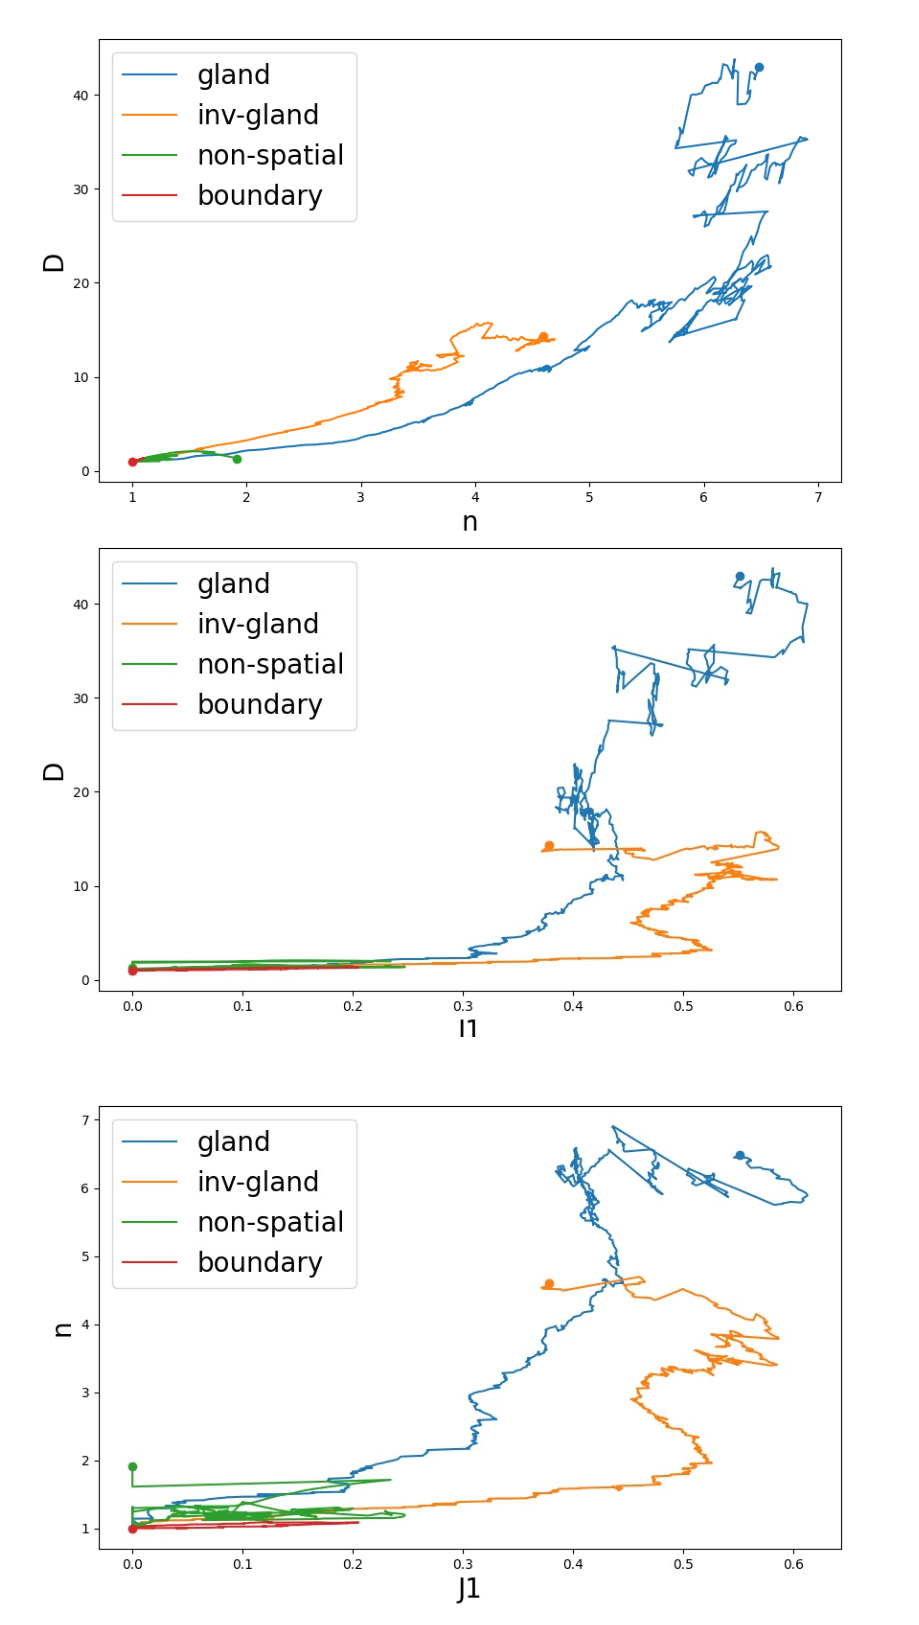
\includegraphics[width=0.85\textwidth]{Chapter_3/figures/1e0501.pdf}
    \caption{Evolutionary trajectories in $3$-dimensional index space for four
    different spatial configurations of tumour progression (gland fission,
    invasive glandular, non-spatial, and boundary growth) averaged over $50$
    replicates each. Parameters: mutation rate $\mu = 10^{-5}$, selective
    advantage $s = 0.1$.}
    \label{fig:1e05_01}
\end{figure}

\begin{figure}[h!]
    \centering
    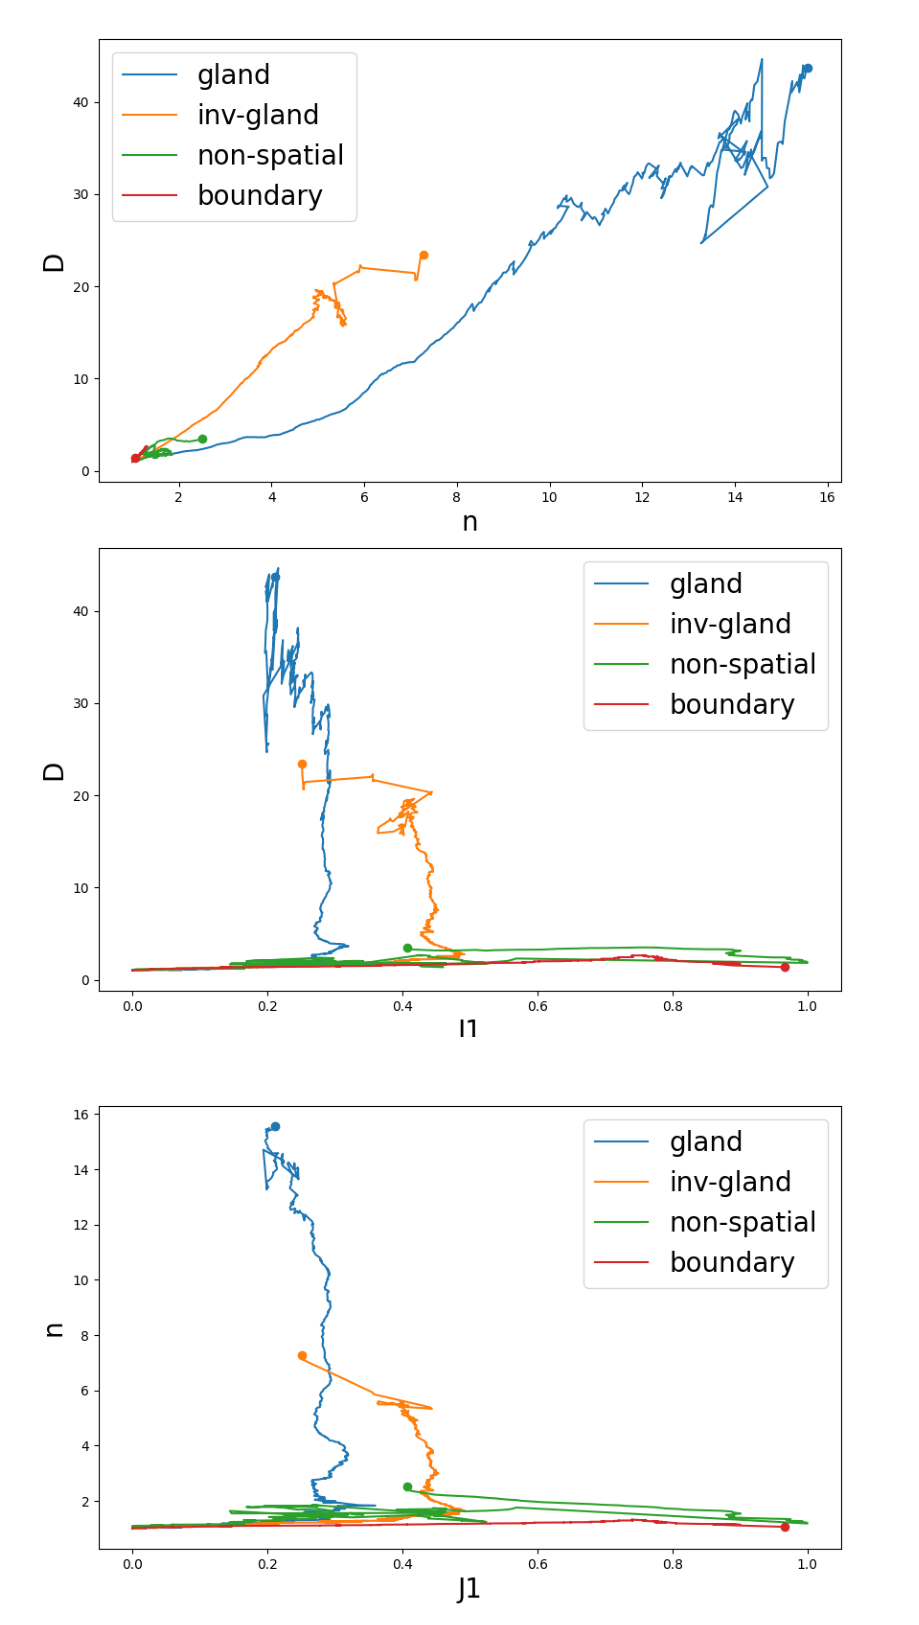
\includegraphics[width=0.85\textwidth]{Chapter_3/figures/1e04005.pdf}
    \caption{Evolutionary trajectories in $3$-dimensional index space for four
    different spatial configurations of tumour progression (gland fission,
    invasive glandular, non-spatial, and boundary growth) averaged over $50$
    replicates each. Parameters: mutation rate $\mu = 10^{-4}$, selective
    advantage $s = 0.05$.}
    \label{fig:1e04_005}
\end{figure}
\clearpage

\subsection{Trajectories in the new index space}
As the $3$-dimensional index space does not distinguish between topologically
identical trees with different branch lengths, I decided to re-run the analysis
on the same set of simulations using a recently introduced system of indices
\cite{noble_new_2023}. Using an early version of the R package for calculating
the indices \cite{kimverity_kimverityruiindices_2023}, I was able to construct
the average trajectories in this new larger index space. However, bigger is not
always better, and there are some redundancies in the new set of indices. For
example, in all cases, the longitudinal and node evenness indices were highly
correlated across runs (figure \ref{fig:evenness_redundant}). Furthermore, the
richness indices were also correlated with the diversity indices, which is not
surprising as the diversity indices are a generalisation of the richness
indices. I will narrow down the the set of indices to just the diversity
indices and one of the evenness indices in this section, with the full set of
trajectories included in appendix \ref{app:trajs}.\par

\begin{figure}[h!]
    \centering
    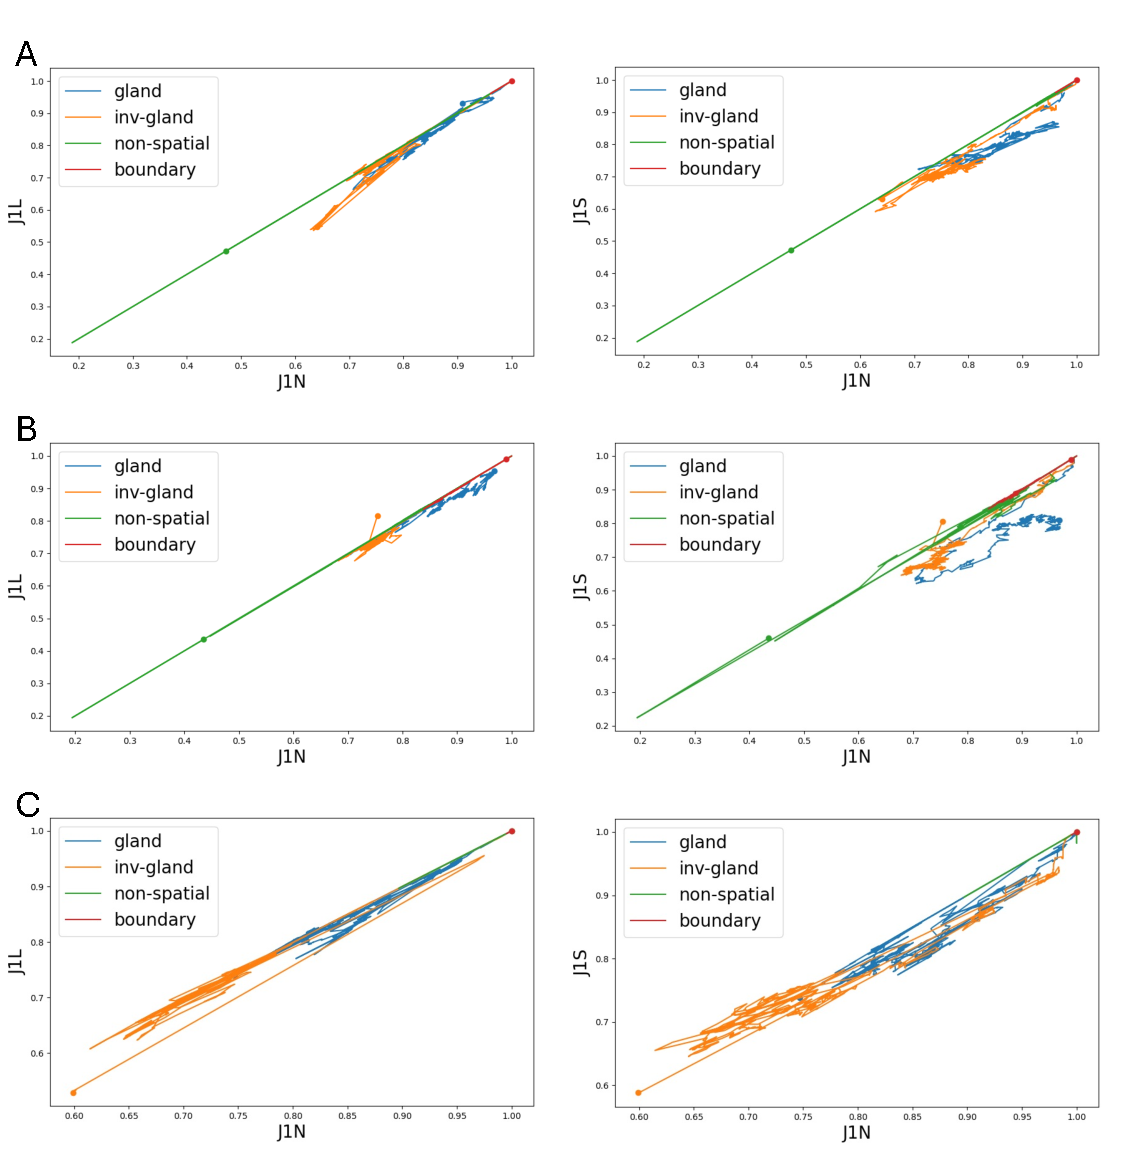
\includegraphics[width=\textwidth]{Chapter_3/figures/redundancy.pdf}
    \caption{Evenness trajectories for different spatial configurations and
    sets of parameters averaged over $50$ replicates each. Mutation rate
    ($\mu$) and selective advantage ($s$) values:\\ \textbf{A} --- $\mu =
    10^{-5}$, $s = 0.1$; \textbf{B} --- $\mu = 10^{-4}$, $s = 0.05$; \textbf{C}
    --- $\mu = 10^{-6}$, $s = 0.2$.}
    \label{fig:evenness_redundant}
\end{figure}
\clearpage

During the analysis, I found that similar patterns emerged in the new index
space as in the old one. Spatial configurations tended to separate into their
own sections of the index space, with overlap present depending on the choice
of parameters. This is not surprising, as the new set of indices is a
generalised version of the old one. The main difference between the new and old
trajectories is the amount of noise present in the new set, even when the
outputs are averaged over multiple runs. This is likely due, in part, to the
inclusion of branch lengths in the new set of indices, which may vary greatly
between runs. The trajectories for the same data sets as above are shown in
figures \ref{fig:1e05_01new} and \ref{fig:1e04_005new}.

\begin{figure}[h!]
    \centering
    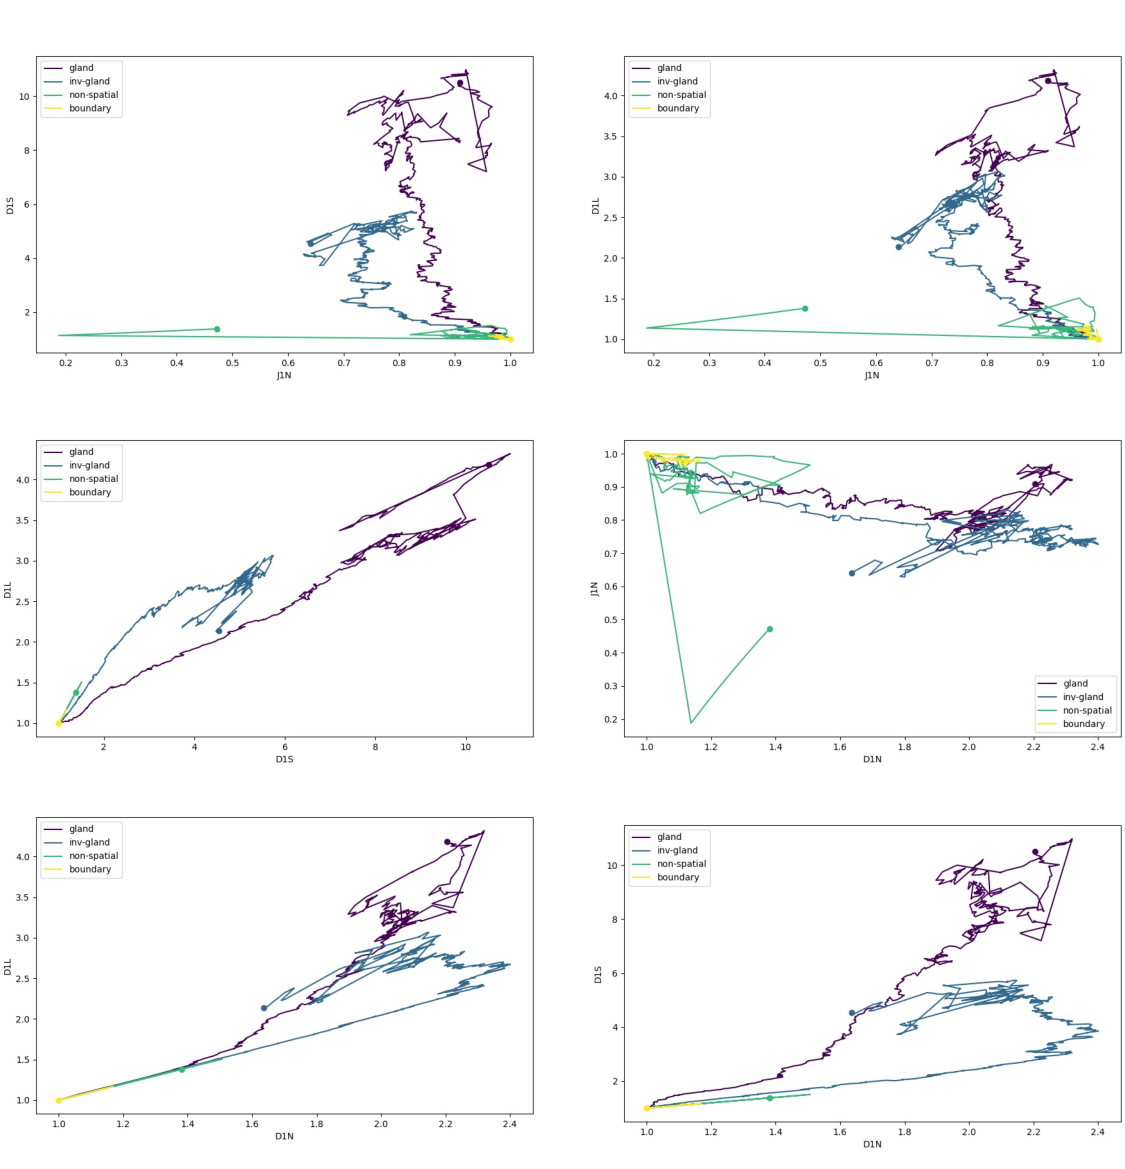
\includegraphics[width=\textwidth]{Chapter_3/figures/1e0501new.pdf}
    \caption{Evolutionary trajectories in the new index space for four
    different spatial configurations of tumour progression (gland fission,
    invasive glandular, non-spatial, and boundary growth) averaged over $50$
    replicates each. Parameters: mutation rate $\mu = 10^{-5}$, selective
    advantage $s = 0.1$.}
    \label{fig:1e05_01new}
\end{figure}
\begin{figure}[h!]
    \centering
    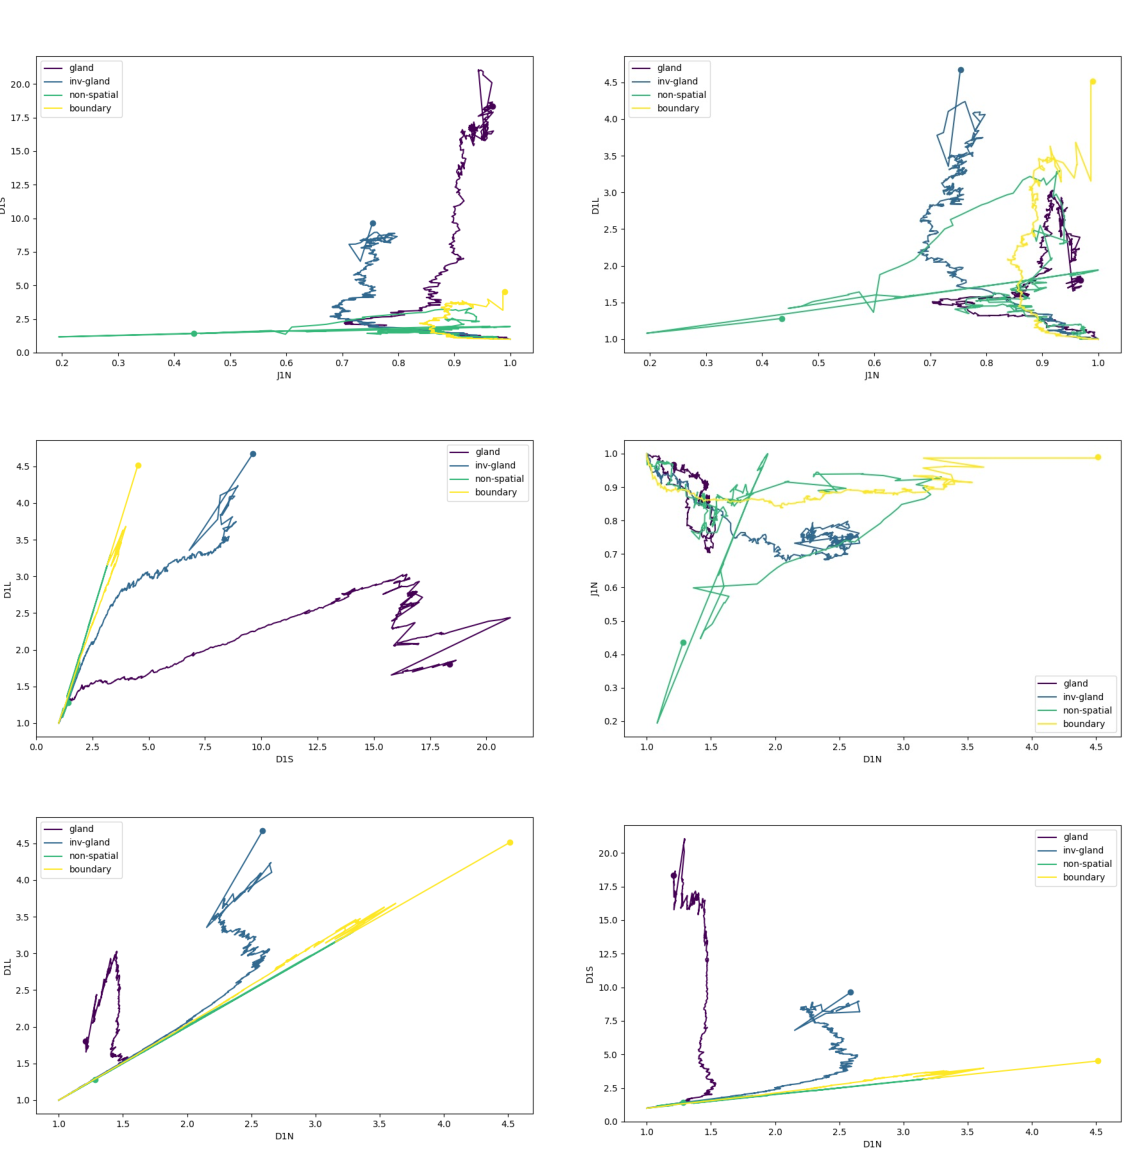
\includegraphics[width=\textwidth]{Chapter_3/figures/1e04005new.pdf}
    \caption{Evolutionary trajectories in the new index space for four
    different spatial configurations of tumour progression (gland fission,
    invasive glandular, non-spatial, and boundary growth) averaged over $50$
    replicates each. Parameters: mutation rate $\mu = 10^{-4}$, selective
    advantage $s = 0.05$.}
    \label{fig:1e04_005new}
\end{figure}
\clearpage

\section{Discussion}
In this chapter I examined two sets of tree shape indices for tracking the mode
of tumour evoution on the example of agent-based simulations. The results
suggest that the indices are able to distinguish between different modes of
evolution depending on parameter choice, but that further work is needed to
establish ranges of parameter values which are useful. While a moderate
mutation rate and weak selection seem to be a good starting point, applying the
indices to real data should be the next step in order to validate the approach.
Furthermore, the new set of indices introduced in \cite{noble_new_2023} is more
informative due to its inclusion of branch lengths, but also
contains some redundancy as pairs of indices can display high correlation
across runs. This redundancy may not necessarily be present in all individual
simulations, but averaging even a few dozen runs shows that pairs of indices
encode similar information. Despite the averaging, there is still a
considerable amount of noise in the derived trajectories, and larger-scale
simulations are needed to produce cleaner results. Additionally, I looked at the
arithmetic mean trajectory for each parameter set which, in retrospect, may not
have been the most informative summary of the data --- considering some form of
median trajectory may have been more representative of the processes in the
simulations. \par
As the new index set is, as the name suggests, new, there are still some
technical wrinkles to iron out. Namely, large trees with many nodes and branches
can take a long time to calculate, as the indices from the set are more complex
than the old ones. Additionally, there is a precision issue which arises when
some of the smallest nodes are included in the tree. This is easily resolved by
employing a similar approach as in \ref{fig:robustness}, which effectively
simulates sampling error. Finally, the R package itself does not directly
support the data structure used in the modelling workflow. The conversion, which
was purpose-written for this work, may also contribute to the aforementioned
technical difficulties. \par

The main contribution of this chapter is the exploration of different sets of
indices, not just over time, but in relation to each other. The first time a
similar approach was used was in \cite{noble_spatial_2022}, and here I expanded
the analysis to include more dimensions of the space. Additionally, in the
context of the new index set, I was able to expand the discussion to include
larger trees than previously analysed with the indices \cite{noble_new_2023}.
Recently, there has been work considering a similar approach for the
classification of evolutionary processes in biogeography, which further supports
the utility of the indices \cite{freitas_patch_2024}. \par

Having focussed on numerical summaries of the ABM outputs, I also believe that
there may be a way to heuristically derive approximate general properties of a
tumour's evolutionary trajectory. This could be done by deriving equations for
the simplest evolutionary trajectories, such as progressive selective sweeps
which follow a cycloid in the $n,D$-plane in the $3$-dimensional index space.
Additionally, as my main focus in this chapter has been the generation,
processing, and visualisation of synthetic cancer data, there is a good scope
for the application of more novel statistical learning methods to the data,
such as evolutionary simulation \cite{herald_autonomous_2022}, or deep learning
methods developed for fitting ABMs to data \cite{cess_fitting_2023}.

